\chapter{Supplementary: thermal forward modelling operator}
\label{c:ThermModel}

The thermal parameter fitting strategy and the obtained thermal model (chapter~\ref{c:ThermAppl}) rely on a finite-difference solver for the steady-state heat equation.
Its fundamental relationship can expressed in the following vector form:
\begin{equation}
    \label{suppl:eq:heateq}
    \bm{\nabla} \cdot ( k(\bm{x}) \bm{\nabla} T(\bm{x}) ) = - A(\bm{x})
\end{equation}
with $k$ thermal conductivity (considered isotropic), $T$ temperature, $A$ heat production per unit of volume, and $\bm{x}$ position vector.
This form results from simplification of the well known heat equation in its full form \parencites{Fourier1822,Carslaw1959}, a heat source term included:
\begin{equation}
    \label{suppl:eq:fullheateq}
    \frac{\partial T}{\partial t} = \alpha \bm{\nabla}^2 T + \frac{A}{\rho c_p}
\end{equation}
where $t$ denotes time and $\alpha$ `thermal diffusivity', i.e. the product of thermal conductivity ($k$), density ($\rho$), and specific heat ($c_p$).
The steady-state assumption imposes:
\begin{equation}
    \label{suppl:eq:steadystate}
    \frac{\partial T}{\partial t} = 0
\end{equation}
This allows simplification of Eq.~\ref{suppl:eq:fullheateq} to:
\begin{equation}
    \label{suppl:eq:steadystatefullheateq}
    0 = \rho c_p \left( k \bm{\nabla}^2 T + A \right)
\end{equation}
therefore:
\begin{equation}
    \label{suppl:eq:steadystatefullheateq_simplified}
    k \bm{\nabla}^2 T = - A
\end{equation}
which is equivalent to Eq.~\ref{suppl:eq:heateq}, as expressed above \parencite[e.g. ][, chapter 3]{stuwe2007geodynamics}.
% NOTE! Not sure if heat equation with a non-uniform k is a Poisson's equation
%This is a partial differential equation (PDE), in the form of Poisson's equation ($\bm{\nabla}^2 \phi = f$, for two generic $\phi$ and $f$ functions).

Analytical solution to this partial differential equation exist: plenty are available for specific cases in the Earth sciences \parencites(see e.g. )()[][chapter 4.6]{Turcotte2014_geodynamics}[][chapter 3.4]{stuwe2007geodynamics}.
As pointed out by \textcite{Gerya2010} a pitfall of analytical methods for PDE solution is that they are "restricted to relatively simple problems" \parencite[][chapter 3.1]{Gerya2010}.
To analytically express the distribution of parameters' fields (e.g. $A$, $k$) is often cumbersome, sometimes impossible.
For the purposes of this thesis, a solver to the steady-state heat equation based on the finite-difference method \parencites()()[][chapter 4.2]{Patankar1980}[][chapter 10]{Gerya2010} was developed.
Resorting to finite differences implies discretising the infinite model continuum on a mesh of points, which describe the geometrical distribution of physical properties in the model, and then substituting the partial differential equations (i.e. the heat equation as in Eq.~\ref{suppl:eq:steadystatefullheateq_simplified} and the equations describing the boundary conditions) at the grid points with linear equations which locally approximate derivatives.
This procedure results in a system of linear equations, which is solved to obtain the value of the unknowns at each of the grid points.

Leaving the thorough description of the mathematical basis of finite differences (FD) and of the fundamentals of their implementation to the works cited above, this supplementary chapter provides a description on the modelling solution devised for the aim of this thesis.

\section[
    tocentry={Finite-difference approximation of the steady-state heat equation},
    head={FD approximation of the steady-state heat equation}
    ]{Finite-difference approximation of the steady-state heat equation}
\label{s:ThermModel:FD}

\FloatBarrier

\begin{figure}[hb] % stencil figure: nodes and grid spacing
    \begin{adjustbox}{center}
        \fbox{
            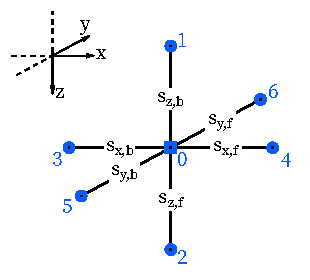
\includegraphics[width=0.7\textwidth]{./0200/grid_stencil_complete.pdf}
        }
    \end{adjustbox}
    \caption[The 7-point stencil used to formulate the central finite differences.]{The 7-point stencil used to formulate the central finite differences for the heat equation around node $0$ (neighbours nodes $1$ to $6$).
    Each $i$-th node corresponds to a value of $T_i$, $k_i$, $A_i$.
    The axis convention is shown in the upper left corner.
    $s_{m,n}$ denotes the grid spacing between nodes, along the $m$-axis and $n$-direction along axis ($b$ backwards, $f$ forwards).}
    \label{suppl:fig:stencil}
\end{figure}

The heat equation under the assumed conditions (Eq.~\ref{suppl:eq:steadystatefullheateq_simplified}) can be formulated using \textit{central finite differences} for a node and its six neighbours in a 3-D rectangular grid.
The 7-node \textit{stencil} of this nodal configuration (i.e. its graphical representation) is shown in Fig.~\ref{suppl:fig:stencil}.

Remembering Fourier's law of heat conduction, which defines heat flux $Q$:
\begin{equation}
    \label{suppl:eq:HeatFlux}
    \bm{Q} = -k \bm{\nabla} T
\end{equation}
we express it in the Leibniz's notation for Cartesian coordinates, which will come useful further in this description:
\begin{equation}
    \label{suppl:eq:HeatFlux_3D}
    \bm{Q} =
        -k \left( 
            \frac{\partial T}{\partial x} \bm{\hat{i}} +
            \frac{\partial T}{\partial y} \bm{\hat{j}} +
            \frac{\partial T}{\partial z} \bm{\hat{k}}
        \right)
\end{equation}
with $\bm{\hat{i}}$, $\bm{\hat{j}}$, $\bm{\hat{k}}$ unit vectors of $x$, $y$, $z$ coordinates.
For the sake of clarity, we indicate each of these heat flux components as $Q_x$, $Q_y$, $Q_z$:
\begin{equation}
    \label{suppl:eq:HeatFlux_3D_component}
    \bm{Q} = 
    \left(-k \frac{\partial T}{\partial x} \bm{\hat{i}} \right) +
    \left(-k \frac{\partial T}{\partial y} \bm{\hat{j}} \right) +
    \left(-k \frac{\partial T}{\partial z} \bm{\hat{k}} \right) = Q_x + Q_y + Q_z
\end{equation}
By substituting this into the $k \bm{\nabla}^2 T$ term of Eq.~\ref{suppl:eq:steadystatefullheateq_simplified}, we get:
\begin{equation}
    \label{suppl:eq:steadystatefullheateq_simplified_Q}
    - \frac{\partial}{\partial x} Q_x -
    \frac{\partial}{\partial x} Q_y -
    \frac{\partial}{\partial x} Q_z = A
\end{equation}
Note that we also flipped the sign of both sides of the equation, to obtain a positive right-hand-side.

Turning to finite differences, Eq.~\ref{suppl:eq:steadystatefullheateq_simplified_Q} can be expressed for each internal node and its 6~neighbours in the model mesh, as illustrated in Fig.~\ref{suppl:fig:stencil}.
Each $i$-th node is characterised with its associated parameters: $T_i$, $k_i$, $A_i$.
On each segment of the graph connecting `node $0$' and its neighbours we add a \textit{staggered node} representing the heat flux between the neighbour and the central node, therefore we have split each component of heat flux $\bm{Q}$ in its backwards and forwards parts, respect to the central node, along the direction defined by each of the unit vectors.
To prevent further cluttering Fig.~\ref{suppl:fig:stencil}, these $Q_{m,n}$ heat flux nodes are represented on a separate stencil, in Fig.~\ref{suppl:fig:stencil_staggered}.

\begin{figure}[ht] % stencil figure: fully staggered nodes
    \begin{adjustbox}{center}
        \fbox{
            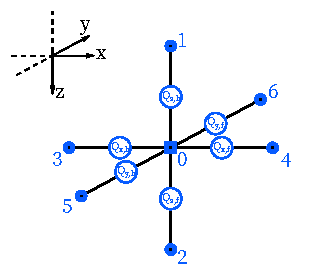
\includegraphics[width=0.7\textwidth]{./0200/grid_stencil_staggered.pdf}
        }
    \end{adjustbox}
    \caption[Additional (staggered) points used in the central finite difference formulation.]{The 6 additional \textit{fully staggered points} used in the central finite difference formulation, where heat fluxes ($Q_{m,n}$) between node $0$ and its neighbours are expressed.
    The $m$ subscript denotes the axis, the $n$ subscript the along-axis direction ($b$ backwards, $f$ forwards).}
    \label{suppl:fig:stencil_staggered}
\end{figure}

Using one of the terms of Eq.~\ref{suppl:eq:steadystatefullheateq_simplified_Q} as an example, this implies that:
\begin{equation}
    \label{suppl:eq:FD_example}
    - \frac{\partial}{\partial x} Q_x \approx
    - \frac{\Delta Q_x}{\Delta x} =
    \frac{-(Q_{x,f} - Q_{x,b})}{(s_{x,b} + s_{x,f}) / 2} =
    2 \frac{Q_{x,b} - Q_{x,f}}{s_{x,b} + s_{x,f}}
\end{equation}
The sketch provided in Fig.~\ref{suppl:fig:stencil_sketch} helps in representing the finite difference approximation just shown in Eq.~\ref{suppl:eq:FD_example}.
In that figure the grid spacings $s_{x,b}$ and $s_{x,f}$ are plotted as sensibly different on purpose, to highlight the the fact that they may be not equal, in the general case.

\begin{figure}[ht] % stencil figure: sketch for FD example, staggered nodes
    \begin{adjustbox}{center}
        \fbox{
            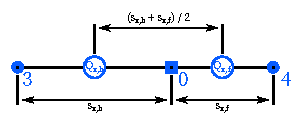
\includegraphics[width=0.7\textwidth]{./0200/grid_stencil_x_sketch.pdf}
        }
    \end{adjustbox}
    \caption[Finite differences around one node, one dimensional sketch.]{One dimensional sketch showing the nodes (basic and staggered) and the spacing distances involved in the FD example of Eq.~\ref{suppl:eq:FD_example}.}
    \label{suppl:fig:stencil_sketch}
\end{figure}

We can now write the FD approximation for the fluxes in Eq.~\ref{suppl:eq:steadystatefullheateq_simplified_Q}:
\begin{equation}
    \label{suppl:eq:FD_fluxes}
    2 \frac{Q_{x,b} - Q_{x,f}}{s_{x,b} + s_{x,f}} +
    2 \frac{Q_{y,b} - Q_{y,f}}{s_{y,b} + s_{y,f}} +
    2 \frac{Q_{z,b} - Q_{y,f}}{s_{z,b} + s_{z,f}} = A_0
\end{equation}

It is now the turn of FD approximation of the $Q_{m,n}$ fluxes at the staggered nodes.
Using node $Q_{x,b}$ an example (see Fig.~\ref{suppl:fig:stencil_sketch_flux} for a sketch):
\begin{equation}
    \label{suppl:eq:FD_staggered_example}
    Q_{x,b} =
    -k_{x,b} \frac{\partial T}{\partial x} \approx
    -k_{x,b} \frac{\Delta T}{\Delta x} =
    -k_{x,b} \frac{T_0 - T_3}{s_{x,b}}
\end{equation}
A value of thermal conductivity at the staggered node has been added ($k_{x,b}$).
It is computed as the arithmetic average between the conductivities of the central node (node~$0$) and its neighbour (node~$3$ in this example):
\begin{equation}
    \label{suppl:eq:FD_staggered_example_conductivity}
    k_{x,b} = \frac{k_0 + k_3}{2}
\end{equation}

\begin{figure}[hb] % stencil figure: sketch for FD example, one flux
    \begin{adjustbox}{center}
        \fbox{
            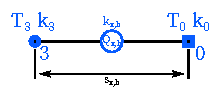
\includegraphics[width=0.525\textwidth]{./0200/grid_stencil_x_sketch_flux.pdf}
        }
    \end{adjustbox}
    \caption[Conservative finite differences: sketch for the staggered node example.]{One dimensional sketch showing the nodes, parameters, and spacing involved in the example of Eq.~\ref{suppl:eq:FD_staggered_example}, the FD approximation of heat flux at a staggered node $Q_{x,b}$.}
    \label{suppl:fig:stencil_sketch_flux}
\end{figure}

By doing so for all the remaining $Q_{m,n}$ fluxes at staggered nodes around node~$0$, Eq.~\ref{suppl:eq:FD_fluxes} becomes:
\begin{align}
\begin{split}
    \label{suppl:eq:FD_fluxes_complete}
    2 \frac{
            \left( -k_{x,b} \displaystyle \frac{T_0 - T_3}{s_{x,b}} \right ) -
            \left( -k_{x,f} \displaystyle \frac{T_4 - T_0}{s_{x,f}} \right )
        }{s_{x,b} + s_{x,f}} &+ \\[1ex]
    2 \frac{
            \left( -k_{y,b} \displaystyle \frac{T_0 - T_5}{s_{y,b}} \right ) -
            \left( -k_{y,f} \displaystyle \frac{T_6 - T_0}{s_{y,f}} \right )
        }{s_{y,b} + s_{y,f}} &+ \\[1ex]
    2 \frac{
            \left( -k_{z,b} \displaystyle \frac{T_0 - T_1}{s_{z,b}} \right ) -
            \left( -k_{z,f} \displaystyle \frac{T_2 - T_0}{s_{z,f}} \right )
        }{s_{z,b} + s_{z,f}} &= A_0
\end{split}
\end{align}
Further expressing the averaged conductivities at staggered nodes $k_{m,n}$, we obtain:
\begin{align}
\begin{split}    
    \label{suppl:eq:FD_fluxes_complete_k}
    2 \frac{
            \left(
                \displaystyle \frac{k_0 + k_3}{2}
                \displaystyle \frac{T_0 - T_3}{s_{x,b}}
            \right ) -
            \left(
                \displaystyle \frac{k_4 + k_0}{2}
                \displaystyle \frac{T_4 - T_0}{s_{x,f}}
            \right )
        }{s_{x,b} + s_{x,f}} &+ \\[1ex]
    2 \frac{
            \left(
                \displaystyle \frac{k_0 + k_5}{2}
                \displaystyle \frac{T_0 - T_5}{s_{y,b}} \right ) -
            \left(
                \displaystyle \frac{k_6 + k_0}{2}
                \displaystyle \frac{T_6 - T_0}{s_{y,f}}
            \right )
        }{s_{y,b} + s_{y,f}} &+ \\[1ex]
    2 \frac{
            \left(
                \displaystyle \frac{k_0 + k_1}{2}
                \displaystyle \frac{T_0 - T_1}{s_{z,b}}
            \right ) -
            \left(
                \displaystyle \frac{k_2 + k_0}{2}
                \displaystyle \frac{T_2 - T_0}{s_{z,f}}
            \right )
        }{s_{z,b} + s_{z,f}} &= A_0
\end{split}
\end{align}

We started with the FD discretisation of fluxes at the central node (Eq.~\ref{suppl:eq:FD_fluxes}), then formulated the FD discretisation of fluxes at staggered nodes (Eq.~\ref{suppl:eq:FD_staggered_example}).
This is called a `conservative finite-difference discretisation', which allows for variable thermal conductivity.
\textcite{Gerya2010} provides a thorough explanation on its rationale, using the Stokes equation with variable viscosity and the Lagrangian heat conservation equation (non-steady state) as examples.

\section[
    tocentry={From the FD formulation to a system of linear equations},
    head={From the FD formulation to a system of linear equations}
    ]{From the finite difference formulation to a system of linear equations}
\label{s:ThermModel:FD_LinSyst}

With the derivation described in the previous section, a finite-difference approximation for the steady-state heat equation was obtained for one node, surrounded by a neighbour in each Cartesian direction.
In order to turn that into a thermal model, we need to transform the FD formulations of each node into a system of linear equations.
In addition, the boundary conditions must be defined and specified in the appropriate form.
The system is in the following form:
\begin{equation}
    \label{suppl:eq:FD_LinSyst_form}
    \bm{L} \bm{T} = \bm{R}
\end{equation}
For a system of $n$ equations (i.e.~$n$ nodes, including those used to impose boundary conditions), $\bm{T}$ is $n$~by~\num{1} vector of unknowns (the sought temperature at each node), $\bm{R}$ is a \num{1}~by~$n$ vector of the right-hand-sides of the equations, and $\bm{L}$ is a $n$~by~$n$ matrix of coefficients which multiply the elements of $T$.
In the FD modelling case of this thesis, $\bm{L}$ is a sparse matrix, i.e. most of its elements are zero.
This is a direct consequence of the 7-nodes stencil that define the parameters of the heat equation in each node: each linear equation, thus each line in matrix $\bm{L}$, has 7 non-zero parameters for inner nodes.
As described afterwards, boundary nodes have one to two non-zero elements in $\bm{L}$, depending on their type.

By expressing an FD model as a system of linear equations (Eq.~\ref{suppl:eq:FD_LinSyst_form}) we can solve for the unknown $\bm{T}$, provided that $\bm{L}$ is nonsingular:
\begin{equation}
    \label{suppl:eq:FD_LinSyst_inversion}
    \bm{T} = \bm{L}^{-1} \bm{R}
\end{equation}

As mentioned when describing the thermal application (chapter~\ref{c:ThermAppl}), for the aim of this thesis $\bm{L}$ was inverted using the \textit{UMFPACK} factorization for sparse matrices \parencite{Davis2006}.
% Providing its description here may be well beyond the scope of this thesis.
In computational terms, it is a direct solver.
For an increasing number of dimensions and model nodes it may result in an unmanageable amount of memory.
The call to a fall-back alternative, an iterative solver \parencite[the generalized minimal residual method, \textit{gmres}, see][]{Saad1986gmres}, has been included in the code, but it never occurred to require resorting to it, in the experiments described here.

\paragraph*{Indexing in the coefficient matrix}
The form of the system (Eq.~\ref{suppl:eq:FD_LinSyst_form}) requires that each $T_i$ that appears in the equation of each node is expressed in a separate term, multiplied by a coefficient $L_i$.
This results in an equation in the general form $\sum (L_i T_i) = R_r$, an equation for each $r$-row of $\bm{L}$.
The coefficients of each equation are then placed in the proper column of $\bm{L}$, i.e. the column corresponding to the element of vector $\bm{T}$ that they multiply.

Using the $r$-th row of the coefficient matrix $\bm{L}$ as an example, expressing the coefficients in the left-hand-side of the equation of the $r$-th node of the model, we can formulate the following.
The coefficient that multiplies the temperature in the $r$-th node is in $L_{r(0),r(0)}$. This is $T_0$ in the heat equation for an inner node (Eq.~\ref{suppl:eq:FD_fluxes_complete_k}).
Leaving the issue of indexing aside for a moment -- for the sake of clarity -- we call $r(i)$ the index related to the $i$-th neighbour in the notation of Eq.~\ref{suppl:eq:FD_fluxes_complete_k}.
The structure of this $r$-th row of $\bm{L}$ will be:
\begin{equation*}
    \setcounter{MaxMatrixCols}{20}
    \label{suppl:eq:FD_LinSyst_RowExampleNoIndex}
    \mathclap{%
    \begin{matrix}
        \cdots & L_{r(0),r(5)} & \cdots & L_{r(0),r(3)} & \cdots & L_{r(0),r(1)} & L_{r(0),r(0)} & L_{r(0),r(2)} & \cdots & L_{r(0),r(4)} & \cdots & L_{(0),r(6)} & \cdots
    \end{matrix}}
\end{equation*}
The ellipses ($\cdots$) indicate zero elements in the sparse matrix.

In order to fill the coefficient matrix, the geometric coordinates of each node in the 3-D mesh must be transformed to a \textit{global index} $r$ that expresses its position in $\bm{T}_r$, $\bm{L}_{r,r}$, $\bm{R}_r$.
This is trivial for a rectilinear mesh, by knowing the number of nodes along each axis ($x_n$, $y_n$, $z_n$) and the defined axis ordering ($z$, then $x$, then $y$, in this case).
The vectors of grid steps along each axis, which are not necessarily constant, are known and provide a linear map between axis coordinates ($z,x,y$) and element along the axis ($u,v,w$).
The \textit{global index} for a node in $u,v,w$ is therefore:
\begin{equation}
    \label{suppl:eq:GlobalIndex}
    r(u,v,w) = (w-1) x_n z_n + (v-1) z_n + u
\end{equation}
when $u,v,w$ are counted starting from \num{1}.
Therefore, moving to the next node:
\begin{itemize}
    \item along $z$ implies changing $r$ by one;
    \item along $x$ implies changing $r$ by $z_n$;
    \item along $y$ implies changing $r$ by $x_n$~times~$z_n$.
\end{itemize}
An example for a 3~$\times$~3 model is shown in Fig.~\ref{suppl:fig:GridIndexing}.

\begin{figure}[h]
    \begin{adjustbox}{center}
        \fbox{
            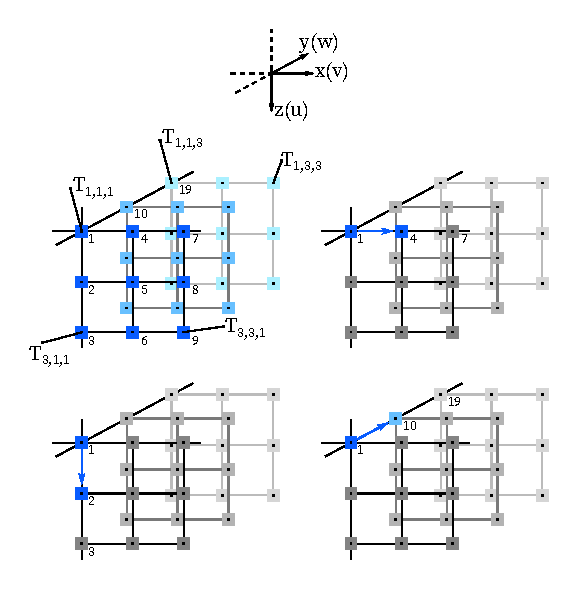
\includegraphics[width=1.1\textwidth]{./0200/grid_indexing.pdf}
        }
    \end{adjustbox}
    \caption[Cartesian coordinates and global indexing on a 3~$\times$~3 mesh.]{Cartesian coordinates and global indexing, illustrated for a 3~$\times$~3 mesh. The value of $r(u,v,w)$ (Eq.~\ref{suppl:eq:GlobalIndex}) is shown beside each node square. Three examples of node-by-node movement are shown.}
    \label{suppl:fig:GridIndexing}
\end{figure}

\FloatBarrier

\paragraph*{Boundary conditions}
Two types of boundary conditions are specified for the nodes at the boundary of the model mesh:
\begin{itemize}
    \item at the top and bottom boundaries, temperature is set: a first-type (Dirichlet) boundary condition in the form $T(\mathrm{boundary}) = T$;
    \item at the vertical boundaries (the sides normal to the $x$ and $y$ axes), zero-flux is set: a second-type (Neumann) boundary condition in the form $\partial T / \partial x = 0$ (where $x$ is the cartesian axis the boundary is normal to).
\end{itemize}

\subparagraph*{First type: boundary temperature}
In the matrix form of the system of linear equations, the first-type boundary condition for the $r$-th node results in the following equation:
\begin{equation}
    \label{suppl:eq:BoundaryT_NodeEq}
    1 \cdot T(r) = T_b
\end{equation}
where $T_b$ is the temperature at the boundary (in this work, either the surface temperature or the lithosphere-asthenosphere boundary temperature).
This results in only one coefficient for the $r$-th row in the coefficient matrix~$\bm{L}$: $\bm{L}_{r,r} = 1$.
In the general case, the topography and the base of the lithosphere are not flat.
This is achieved by imposing the same condition, using coefficients, to all the inner mesh nodes at and above the topography and at and below the lithosphere-asthenosphere boundary.
An alternative formulation for the bottom boundary is to provide it flat with a varying temperature -- this use case, which was implemented but not employed in this work, allows to use the type of depth-slice data which can be inferred from e.g. seismic tomography.
As a side note, the physical meaning of this type of boundary, in steady state, is that the heat transfer and heat production from the base of the lithosphere to the topography is not increasing the temperature of the atmosphere (or ocean) above the latter, nor decreasing the temperature of the asthenosphere beneath the former -- this is a fundamental assumption of steady state thermal modelling.

\subparagraph*{Second type: no heat flux boundary}
Imposing a zero heat flux means that no temperature gradient should be present across the boundary: i.e. given a temperature $T_0$ at the boundary node (global index $r_0$) and a temperature $T_1$ at an additional node outside the boundary (global index $r_1$), then $T_0 - T_1 = 0$.
In the matrix form of the system of linear equations, this results in:
\begin{equation}
    \label{suppl:eq:BoundaryQ_NodeEq}
    1 \cdot T(r_0) - 1 \cdot T(r_1) = 0
\end{equation}
Thus we now have two coefficients for the $r_0$-th row in the coefficient matrix~$\bm{L}$: $\bm{L}_{r_0,r_0} = 1$ and $\bm{L}_{r_0,r_1} = -1$.
Note that zero horizontal flux would be observed for a model which is infinitely uniform along the zero-flux axis.
This implies that 2-D `sections' or 1-D `columns' can be also modelled with this 3-D implementation, provided that the mesh is built accordingly.

\paragraph*{FD heat equation coefficients}

% C'È PASSAGGIO A ESPLICITO, PER AVERE COEFFICIENTI CHE MOLTIPLICANO T
% ADESSO ATTENZIONE A DISCORSO VARIABLE STEP, VEDO APPUNTI!
% qui soluzione, anche se lunga (tutta esplicita)

% figura "spy" con elementi non-zero (fare esempi, fermando il solver)
% provo una cross-correlation matrix a posteriori, del modello?

% valutare se le successive sono necessarie
%\section{Matlab implementation}
%\label{s:ThermModel:Implementation}

% vectorized global index
% identificazione dei boundary

% \section{Definition of lithospheric volumes}
% \label{s:ThermModel:MakeVol}
